\section{What is a quantum dot?}
\label{sec:quantum-dot-introduction}

A quantum dot is a small region in a material that confines electrons
in all three spatial directions. A potential well provides a useful
picture: an electron has lower potential energy inside the region and
must cross an energy barrier to leave it. The localized spatial states
of the electron are its \emph{orbitals}, with discrete energies set by
the size and shape of the well. A dot can contain one electron or several;
confinement makes a small electronic system with its own states and
energy levels. This is the origin of the description of quantum dots
as artificial atoms~\cite{Oosterkamp1998}.

These notes consider quantum dots in crystalline \emph{silicon}, a
semiconductor. Metal electrodes held at chosen voltages create electric
fields in the silicon and shape the potential energy of its mobile
electrons. These electrodes are called \emph{gates}, and the resulting
localized electronic region is a \emph{gate-defined quantum dot}.
The well occupies a small part of a continuous piece of silicon.
Changing the gate voltages changes its energy levels and the barriers
around it, allowing us to control which electrons it holds and how
strongly they couple to electrons elsewhere in the device.

\subsection{How gates form a dot}

Figure~\ref{fig:platform-device-section} shows a silicon surface covered
by an insulating layer of silicon dioxide, with metal gates above it.
We take $z$ perpendicular to the interface and $x,y$ along it. To make
a dot, the device must first confine electrons near the interface in
$z$ and then restrict them to a small region in the $x,y$ plane.

The two parts of this confinement have different physical origins.
An electron in the silicon encounters a high material energy barrier
at the oxide. A suitable gate voltage lowers the electron's energy
near the interface relative to the silicon farther below it. The
oxide barrier on one side and the rising energy into the silicon on
the other form a well in $z$. The shapes and voltages of the gates
also make the potential vary along the interface. A lateral minimum
surrounded by barriers then confines the electron in $x$ and $y$,
completing the three-dimensional well~\cite{Zwanenburg2013}.

The voltage of each gate is set by an external source. Through the
electric field, this voltage changes the electric potential $\Phi$
in the silicon and hence the potential energy $-e\Phi$ of an electron,
whose charge is $-e$ with $e>0$. The insulating oxide separates the
gate from the electrons. Electrons are supplied through the contact
on the left of the figure, which connects to a much larger populated
region of silicon. This region serves as an \emph{electron reservoir}:
it can give up or accept one electron with negligible change in its
macroscopic state. The accumulation gate helps populate this region
by lowering the electron potential energy beneath it.

\begin{figure}[!t]
 \centering
 % Idealized reservoir--dot cross-section and matching potential profile.
% Coordinates are in millimetres.
\begingroup
\small
\setlength{\unitlength}{1mm}
\linethickness{0.4pt}
\begin{picture}(150,123)
 \put(0,117){\makebox(150,5)[l]{\bfseries (a) Material cross-section}}

 % Material fills.
 \put(12,63){\color{blue!3}\rule{126mm}{27mm}}
 \put(26,90){\color{black!7}\rule{112mm}{7mm}}
 \put(12,84){\color{black!25}\rule{14mm}{13mm}}
 \put(34,97){\color{black!15}\rule{39mm}{10mm}}
 \put(81,97){\color{black!15}\rule{16mm}{10mm}}
 \put(108,97){\color{black!15}\rule{27mm}{10mm}}

 % Shared material boundaries, drawn once at their exact coordinates.
 \put(12,63){\line(1,0){126}}
 \put(12,63){\line(0,1){34}}
 \put(138,63){\line(0,1){34}}
 \put(26,90){\line(1,0){112}}
 \put(12,97){\line(1,0){126}}
 \put(12,84){\line(1,0){14}}
 \put(26,84){\line(0,1){13}}

 % Gate sides and tops share the oxide top at y=97.
 \put(34,97){\line(0,1){10}}
 \put(73,97){\line(0,1){10}}
 \put(34,107){\line(1,0){39}}
 \put(81,97){\line(0,1){10}}
 \put(97,97){\line(0,1){10}}
 \put(81,107){\line(1,0){16}}
 \put(108,97){\line(0,1){10}}
 \put(135,97){\line(0,1){10}}
 \put(108,107){\line(1,0){27}}

 \put(64,91){\makebox(56,5){insulating oxide}}
 \put(17,65){\makebox(24,5)[l]{silicon}}
 \put(12,84){\makebox(14,13){contact}}
 \put(34,97){\makebox(39,10){\shortstack{accumulation\\gate}}}
 \put(81,97){\makebox(16,10){\shortstack{barrier\\gate}}}
 \put(108,97){\makebox(27,10){\shortstack{plunger\\gate}}}

 % Populated layer and localized orbital; labels sit inside their regions.
 \put(26,84){\color{blue!23}\rule{48mm}{5mm}}
 \put(26,84){\makebox(48,5){reservoir}}
 \put(122,86){\color{orange!75!black}\oval(21,6)}
 \put(111.5,83){\makebox(21,6){dot}}
 \put(77,87){\color{blue!65!black}\vector(1,0){31}}
 \put(108,84){\color{blue!65!black}\vector(-1,0){31}}
 \put(77,78){\makebox(32,5){tunneling}}
 \put(145,77){\vector(0,1){20}}
 \put(143,98){\makebox(6,5){$z$}}
 \put(111,58){\vector(1,0){25}}
 \put(139,55){\makebox(6,5){$x$}}

 \put(0,48){\makebox(150,5)[l]{\bfseries
                              (b) Electron potential energy along the layer}}
 \put(18,6){\vector(1,0){122}}
 \put(18,6){\vector(0,1){35}}
 \put(0,37){\makebox(16,7){$V_{\mathrm{conf}}$}}
 \put(141,3){\makebox(6,5){$x$}}
 \put(36,27){\makebox(36,5){reservoir}}
 \put(77,41){\makebox(26,5){barrier}}
 \put(111,7){\makebox(26,5){dot well}}
 \linethickness{0.8pt}
 \color{blue!65!black}
 \put(27,24){\line(1,0){38}}
 \qbezier(65,24)(76,24)(82,33)
 \qbezier(82,33)(86,40)(90,40)
 \qbezier(90,40)(98,40)(106,24)
 \qbezier(106,24)(114,13)(122,13)
 \qbezier(122,13)(132,13)(137,35)

 % Discrete orbital energies, schematic within the displayed dot well.
 \linethickness{0.65pt}
 \color{orange!75!black}
 \put(112,18){\line(1,0){18}}
 \put(107.5,23){\line(1,0){25.3}}
 \color{black}
 \put(137,15.5){\makebox(10,5)[l]{$\epsilon_0$}}
 \put(137,20.5){\makebox(10,5)[l]{$\epsilon_1$}}
\end{picture}
\endgroup

 \caption{Confinement and electron access in a silicon
 metal--oxide--semiconductor device. (a) The gates act through the
 insulating oxide to shape the electron potential in the silicon.
 Electrons reach the reservoir through the contact and the dot
 through a tunable tunneling barrier. The transverse $y$ direction
 is omitted. (b) A lateral cut through the confining potential shows
 the reservoir, barrier, and dot well. The lines $\epsilon_0$ and
 $\epsilon_1$ indicate discrete orbital energies schematically;
 the actual levels depend on confinement in all three directions.}
 \label{fig:platform-device-section}
\end{figure}
\FloatBarrier

Electrons pass between the reservoir and the dot by tunneling through
the intervening barrier within the silicon. The \emph{barrier gate}
primarily changes the height of this barrier and therefore the
tunneling rate. The \emph{plunger gate} primarily shifts the dot's
energy levels, changing the energy cost of putting an electron there.
These roles explain how the same device can admit an electron and
then retain it: adjust the dot levels to allow loading, and raise
the reservoir barrier to suppress escape. Section~\ref{sec:electron-number-control}
gives the energy conditions that select a particular electron number.
Gate fields overlap, so the names describe the main intended effects
rather than perfectly independent controls.

The stack of metal, oxide, and semiconductor in the figure gives this
structure its name, \emph{MOS}. Another common structure uses a thin
silicon layer between silicon--germanium layers. An electron has lower
energy in the silicon layer, which therefore supplies a vertical well;
gates again provide lateral confinement~\cite{Zajac2015}. In either
case, we describe the total confining potential energy by
$V_{\mathrm{conf}}(\mathbf r)$, combining the material energy offsets
with the electrostatic contribution $-e\Phi(\mathbf r)$
(Appendix~\ref{app:device-confinement}).

\subsection{The states of one confined electron}

The well determines where an electron is localized. To calculate its
orbitals and their energies, we also need its kinetic energy in the
silicon crystal. The periodic lattice changes the relation between
energy and wave vector from that of an electron in vacuum. For the
mobile electrons of interest, this relation is the conduction-band
dispersion $E_{\mathrm c}(\mathbf k)$. In silicon it has several
minima at different wave vectors. The states near each minimum form
a \emph{valley}; different valleys thus describe different crystal
components available to an electron in the same dot
(Fig.~\ref{fig:silicon-band-valleys}).

Figure~\ref{fig:silicon-band-valleys}(a) shows calculated bands of
bulk silicon along a path in wave-vector space. The point $\Gamma$
is $\mathbf k=0$; $X$ and $L$ lie at the boundary of the first
Brillouin zone along the crystal directions $[100]$ and $[111]$,
respectively. The lowest conduction band has a minimum between
$\Gamma$ and $X$. In unstrained bulk silicon, crystal symmetry gives
six equivalent minima along the positive and negative $[100]$,
$[010]$, and $[001]$ directions~\cite{Smith2017Donor}.
Panel (b) locates these six valleys; the $\Gamma$--$X$ segment in
panel (a) passes through one of them. These are crystal directions
and need not coincide with the device axes $x,y,z$.

\begin{figure}[htbp]
  \centering
  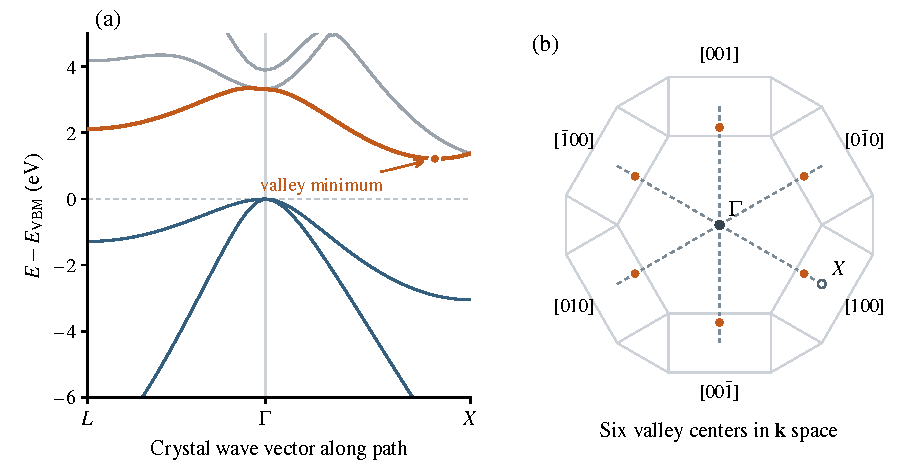
\includegraphics[width=\textwidth]{figures/silicon-band-valleys.pdf}
  \caption{Silicon bands and valleys.
  (a) HSE06 band energies for bulk diamond silicon, replotted from
  NIST JARVIS-DFT record JVASP-1002~\cite{JARVISSiHSE2026}.
  The valence-band maximum is the energy zero. Blue curves show
  valence bands; the lowest conduction band is orange and higher
  conduction bands are gray. The dot marks the sampled minimum
  between $\Gamma$ and $X$.
  (b) Positions of the six symmetry-equivalent valley centers
  (orange dots) in crystal wave-vector space. The wireframe outlines
  the first Brillouin zone; dashed lines point along the six crystal
  directions. This panel shows positions, not energy surfaces.}
  \label{fig:silicon-band-valleys}
\end{figure}
\FloatBarrier

First consider states near one minimum, at $\mathbf k_0$.
The dispersion is approximately quadratic there, so its curvature
defines an inverse effective-mass tensor
(Appendix~\ref{app:effective-mass}):
\begin{equation}
  (\mathbf M^{-1})_{\alpha\beta}
      =\frac{1}{\hbar^2}
        \left.\frac{\partial^2E_{\mathrm c}}
                     {\partial k_\alpha\partial k_\beta}
        \right|_{\mathbf k_0},
  \qquad \alpha,\beta=x,y,z.
  \label{eq:dot-band-curvature}
\end{equation}
Here $\mathbf M$ is the effective-mass tensor of the chosen valley;
it is constant in this uniform-crystal model. Its components are
written in the device coordinates $x,y,z$ defined above and need
not form a diagonal matrix.\footnote{The principal axes are the
eigenvector directions of $\mathbf M$ and need not coincide with the
device axes. Isotropy is the special case $\mathbf M=m^*\mathbf I$,
where $\mathbf I$ is the three-dimensional identity matrix.}

For confinement that varies slowly on the scale of a crystal unit
cell, we can separate the rapid spatial variation of the crystal
state from the variation across the dot. To leading order, the
spatial wave function of a confined electron has the form
\[
  \psi_n(\mathbf r)\simeq
       \chi_{\mathrm c}(\mathbf r)\phi_n(\mathbf r).
\]
Here $\chi_{\mathrm c}$ is the extended crystal state at the chosen
band minimum, while $\phi_n$ is a slowly varying, localized
\emph{envelope}; the index $n$ labels the dot orbitals. The envelope
sets the extent and shape of the electron's probability distribution
across the dot, retaining the crystal structure in $\chi_{\mathrm c}$.

Within this valley, for energies near the minimum and weak
admixture of other bands, the effective-mass reduction derived in
Appendix~\ref{app:effective-mass} gives the envelope equation
\begin{equation}
  \underbrace{
    \left[-\frac{\hbar^2}{2}\sum_{\alpha,\beta}
             (\mathbf M^{-1})_{\alpha\beta}
             \partial_{r_\alpha}\partial_{r_\beta}
          +V_{\mathrm{conf}}(\mathbf r)\right]
  }_{h_0}\phi_n=\epsilon_n\phi_n.
  \label{eq:dot-orbital-eigenproblem}
\end{equation}
Thus the orbital problem is a three-dimensional Schr\"odinger
equation with the effective-mass tensor and the device potential. The energy
of the reference crystal minimum is chosen as the zero; material
offsets and voltage shifts remain in $V_{\mathrm{conf}}$. We will use
the same reference for the dot and reservoir energies. The lowest
solution $\phi_0$ has energy $\epsilon_0$, and higher solutions describe
excited orbitals such as the level $\epsilon_1$ in
Fig.~\ref{fig:platform-device-section}(b).
Their spacing is set by confinement; for example, reducing the size
of a well increases the kinetic energy required for spatial variation
and typically increases the orbital gaps. Weak tunneling to the
reservoir allows us to treat these localized levels as states of
the dot.

The silicon--oxide or silicon--germanium interfaces that provide
vertical confinement also affect the valley states. Their potential
varies on the atomic scale and can couple crystal components near
different band minima~\cite{Friesen2010}. Thus the single-valley
orbital equation supplies one part of the electron's spatial
description. To determine the low-energy states, we must include
the interface coupling between the retained valleys.

For $N_v$ retained valleys, collect the spatial envelopes into
$\mathbf F=(F_1,\ldots,F_{N_v})^{\mathsf T}$.
The multivalley model in Appendix~\ref{app:valley-states} gives
the block Hamiltonian acting on these components:
\begin{equation}
 h_{\mathrm{mv}}=
 \begin{pmatrix}
  h_{0,1} & \hat v_{12} & \cdots & \hat v_{1,N_v}\\
  \hat v_{21} & h_{0,2} & \cdots & \hat v_{2,N_v}\\
  \vdots & \vdots & \ddots & \vdots\\
  \hat v_{N_v,1} & \hat v_{N_v,2} & \cdots & h_{0,N_v}
 \end{pmatrix}.
 \label{eq:dot-coupled-valley-equations}
\end{equation}
Each diagonal block $h_{0,\nu}$ is the orbital Hamiltonian
of Eq.~\eqref{eq:dot-orbital-eigenproblem} for valley $\nu$,
with its own effective-mass tensor and confining potential.
The off-diagonal block $\hat v_{\nu\nu'}$ transfers amplitude
from valley $\nu'$ to valley $\nu$, with
$\hat v_{\nu'\nu}=\hat v_{\nu\nu'}^\dagger$.
In the local model used here, it multiplies the spatial envelope
by a coupling function $v_{\nu\nu'}(\mathbf r)$. These functions
encode the microscopic interface structure and are additional
inputs to the effective model. The eigenstates of
$h_{\mathrm{mv}}$ are combined orbital--valley states; we denote
the lowest one by $\ket{\chi_0}$.

The consequence is particularly simple when the two lowest valleys
are equivalent and share a ground orbital $\phi_0$ of energy
$\epsilon_0$. Assume that all other orbital--valley states lie
higher in energy and that coupling to them is small compared with
their separation from this pair. Projection onto this orbital gives the valley
Hamiltonian (Appendix~\ref{app:valley-states})
\begin{equation}
 H_{\mathrm v}=\epsilon_0 I+
   \begin{pmatrix}0&v_0\\v_0^*&0\end{pmatrix}
 \quad\text{in the basis }(\ket{\nu_1},\ket{\nu_2}),
 \label{eq:dot-valley-doublet}
\end{equation}
where $v_0$ is the interface coupling matrix element within
$\phi_0$. For $v_0=|v_0|e^{i\theta_{\mathrm v}}\ne0$, the
eigenstates, energies, and valley gap are
\begin{equation}
 \begin{aligned}
  \ket{v_\pm}
    &=\frac{\ket{\nu_1}\pm e^{-i\theta_{\mathrm v}}\ket{\nu_2}}
            {\sqrt2},
  &\epsilon_\pm&=\epsilon_0\pm|v_0|,\\
  \Delta_{\mathrm{val}}&=\epsilon_+-\epsilon_-=2|v_0|.
 \end{aligned}
 \label{eq:dot-valley-eigenstates}
\end{equation}
In this limit, the lowest spatial state is
$\ket{\chi_0}=\ket{\phi_0}\otimes\ket{v_-}$. The coupling
can be small compared with an orbital excitation energy while
still determining the valley eigenstates and their entire splitting.
If mixing with excited orbitals is appreciable, the full
Hamiltonian~\eqref{eq:dot-coupled-valley-equations} determines
$\ket{\chi_0}$ and the excitation gaps without assuming this
product form.

Each spatial state also carries the electron's spin. When a common
orbital basis can be used for the retained valleys and spin-dependent
mixing is weak, we can organize the one-electron states as
\begin{equation}
  \Hilb_{N=1}\simeq
  \Hilb_{\mathrm{orb}}\otimes
  \Hilb_{\mathrm{val}}\otimes
  \mathbb{C}^{2}_{\mathrm{spin}}.
  \label{eq:single-electron-space}
\end{equation}
The first factor describes orbital envelopes, the second the
retained valley components, and the third the spin. The coupled
eigenstates need not factor into these parts. To use a single
electron as a spin qubit, we retain the lowest combined spatial
state $\ket{\chi_0}$ and use its two spin states.
Section~\ref{sec:platform-encoding} gives the conditions under
which thermal excitation and control pulses leave the electron
in that spatial state.

\subsection{When the dot contains several electrons}

Several electrons in the same well share the available one-electron
states and repel one another. Their allowed states must also satisfy
fermionic antisymmetry. The energy of an $N$-electron dot therefore
depends both on its one-electron spectrum and on the interaction
between each pair of electrons.

Let $h_1$ be the one-electron Hamiltonian acting on the orbital, valley,
and spin states retained in the description, including any relevant
valley mixing and spin-dependent energies. With spin-dependent
terms omitted, $h_1=h_{\mathrm{mv}}\otimes I_{\mathrm{spin}}$,
where $h_{\mathrm{mv}}$ is the coupled Hamiltonian in
Eq.~\eqref{eq:dot-coupled-valley-equations} and
$I_{\mathrm{spin}}$ is the identity on the two spin states.
The pair interaction $W(\mathbf r,\mathbf r')$ includes the dielectric
and conductor response to the electron charges
(Appendix~\ref{app:screened-interaction}). For $N$ electrons, this
screened repulsion gives the many-electron Hamiltonian
\begin{equation}
  H_N=\sum_{a=1}^{N}h_1^{(a)}
       +\sum_{a<b}W(\mathbf r_a,\mathbf r_b),
  \label{eq:dot-interacting-hamiltonian}
\end{equation}
where $h_1^{(a)}$ acts on electron $a$, and the second sum counts
each interacting pair once.

At fixed gate voltages and other external fields, let $E_N$ denote
the ground-state energy of $H_N$ in the antisymmetric $N$-electron
state space. The resulting sequence $E_0,E_1,E_2,\ldots$
describes the lowest energy available at each electron number.
Which number is actually occupied depends on the energy gained or
lost when electrons are exchanged with the reservoir. That comparison
is developed in Section~\ref{sec:electron-number-control}.

\subsection{Several coupled quantum dots}
\label{sec:multiple-quantum-dots}

Gate electrodes can create several potential minima, each surrounded
by barriers, in the same silicon region. We label the resulting
dots by $i$. Orthonormal localized orbitals provide a basis for specifying how
many electrons occupy each dot; several orbital--valley states and
their spin states can be retained on each dot. The barriers control
electron tunneling between dots, while Coulomb interactions act
both within and between them.

For an array isolated from reservoirs, fix the total electron number
$N$, and write $N_i$ for the number on dot $i$, so that
$N_1+N_2+\cdots=N$. The occupation tuple
$\mathbf N=(N_1,N_2,\ldots)$ defines the subspace
$\Hilb_{(N_1,N_2,\ldots)}$. The single index in $\Hilb_N$
fixes only the total number, while the tuple specifies the number
on every dot. For example, the two-electron space $\Hilb_2$ of
two dots splits into $\Hilb_{(1,1)}$, $\Hilb_{(2,0)}$, and
$\Hilb_{(0,2)}$. Each subspace contains the allowed orbital,
valley, and spin states at those occupations. In this local basis,
grouping the many-electron Hamiltonian by charge configuration
(Appendix~\ref{sec:device-orbital-basis}) gives
\begin{equation}
 \begin{aligned}
  \Hilb_N&=\bigoplus_{N_1+N_2+\cdots=N}
                 \Hilb_{(N_1,N_2,\ldots)},\\
  H_N^{(0)}&=\bigoplus_{N_1+N_2+\cdots=N}
                 H_{(N_1,N_2,\ldots)},
  \qquad H_N=H_N^{(0)}+\mathcal T.
 \end{aligned}
 \label{eq:dot-charge-blocks}
\end{equation}
Both direct sums run over the allowed occupation tuples with total
$N$. Each block $H_{(N_1,N_2,\ldots)}$ acts within the subspace with
that same tuple, and $\mathcal T$ transfers charge between different
subspaces. The superscript $(0)$ denotes the reference with these
transfers omitted. Each block then has its own ground energy
$E_{\mathbf N,0}$ and excited energies $E_{\mathbf N,a}$; the first
energy index labels the occupation tuple, and $a$ labels a level
within that subspace. These energies include the interactions
between electrons on different dots. Thus even when tunneling is
suppressed, the array need not behave as independent dots.

Restoring tunneling couples states in different charge subspaces
while preserving $N$. For two such states with uncoupled energies
$E_{\mathbf N,a}$ and $E_{\mathbf N',b}$, mixing is small when their
coupling matrix element is much smaller than
$|E_{\mathbf N,a}-E_{\mathbf N',b}|$. This is the regime used to keep
local occupations nearly fixed when the relevant charge-transfer
channels are weakly mixed. Near a degeneracy, even a small
nonzero tunnel matrix element can strongly mix the two states.
In a general orbital model, interaction terms can also transfer
charge; they belong to $\mathcal T$ along with single-electron
hopping, as detailed in Appendix~\ref{sec:device-orbital-basis}.

For a simple example, take one electron in two dots. Retain only
the lowest localized spatial state on each dot and a common fixed
spin state, assuming that coupling to other orbital--valley and spin
states can be neglected. Denote the retained states by
$\ket{1,0}$ and $\ket{0,1}$. The local-basis matrix elements in
Appendix~\ref{sec:device-orbital-basis} give
\begin{equation}
 h_{\mathrm{pair}}=
 \begin{pmatrix}
  \epsilon_1&-t_{12}\\
  -t_{12}^*&\epsilon_2
 \end{pmatrix}
 \quad\text{in the basis }(\ket{1,0},\ket{0,1}).
 \label{eq:dot-pair-hamiltonian}
\end{equation}
The diagonal entries are the energies of the two localized states,
and $t_{12}$ is their tunnel coupling, with units of energy. Gate
voltages tune both the detuning $\epsilon_1-\epsilon_2$ and the
barrier that controls $t_{12}$.
When $|\epsilon_1-\epsilon_2|\gg|t_{12}|$, each eigenstate lies
mostly in one charge subspace. When the detuning becomes comparable
to or smaller than $|t_{12}|$, both occupations contribute
appreciably. At $\epsilon_1=\epsilon_2$ and $t_{12}\ne0$, the two
eigenstates have equal weights in $(1,0)$ and $(0,1)$, with energy
separation $2|t_{12}|$ (Appendix~\ref{sec:device-orbital-basis}).
Small tunneling can therefore coexist with strong mixing near
resonance; its magnitude still sets the small splitting and the
associated slow coherent transfer.

